\documentclass[../main.tex]{subfiles}
\graphicspath{{\subfix{../images/}}}

\begin{document}
\textbf{Hello world!}

\begin{figure}[bh]
\centering
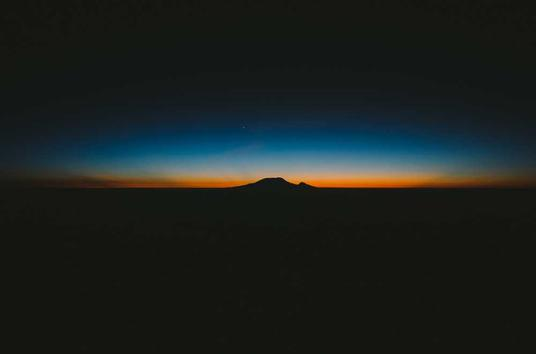
\includegraphics[width=3cm]{picsum lorem}

\label{fig:picsum lorem}
\caption{Overleaf picsum lorem}
\end{figure}

Lorem Ipsum bla\autocite[10]{smith2018} bla bla As stated by 
blas bla bla 

Here we talk about the \gls{ml} and the \gls{ai} in detail.\\ and \gls{ml}
Wie im Aktiengesetz 

Ein Beispieltext mit einem Gesetzeszitat \lawcite[§ 164 Absatz 1 Satz 1]{aktg1965}.


Test Test \autocite[10]{johnson2020}

\medskip

Beispieltabelle: 


\begin{table}
    \centering
    \begin{tabular}{cc}
        Test & Test2\\
        Test3 & Test4\\
    \end{tabular}
    \caption{Caption}
    \label{tab:my_label}
\end{table}
 

\end{document}